\documentclass[10pt]{article}
\usepackage[letterpaper,margin=0.95in]{geometry}
\usepackage{booktabs}
\usepackage{array}
\usepackage{microtype}
\usepackage{parskip}
\usepackage[hidelinks]{hyperref}
\usepackage{enumitem}
\usepackage{graphicx}

\newcommand{\code}[1]{\texttt{#1}}

\title{TAPLite Kernel Computational-Efficiency Enhancements:\\
Warm Starts, SP-Tree Sharing, and Column Stores}
\author{Xuesong Zhou \and TAPLite4MPO team}
\date{July 2026}

\begin{document}
\maketitle

\begin{abstract}
\noindent This memo summarizes the computational-efficiency track for the TAPLite
static-assignment kernel: a five-persona industry panel study that produced a
four-level warm-start ladder (L1--L4); the shipped P0 trio (congested-times warm
start, shortest-path tree sharing, zero-demand-origin skip); the shipped P1
flow restart with a demand-fingerprint guard; and the shipped P2/L3 binary
column store with $\theta$-share warm start and fixed-policy
gradient-projection (GP) sweeps. All shipped features are bit-exact or
exact-with-clearly-reported deviation, default-off where they change behavior,
and gated by a 13-network / 30-check regression suite passed with no
re-baselining. Headline, SCAG RTP24 AM (246{,}806 links, perturbed demand,
same-gap compute): the L3 column warm start reaches a 0.10\% TRUE relative gap
\textbf{139x} faster than a cold run and 0.05\% \textbf{8.4x} faster; targets
at or below 0.02\% are reachable \emph{only} via the GP sweeps --- plain FW,
cold or warm-started, plateaus near 0.03\% while GP reaches
$8\times10^{-4}$\,\%. The standard rerun recipe is therefore an L3 warm start
with a 0.1\% gap target.
\end{abstract}

\section{Headline numbers for the 4-step feedback loop}
\label{sec:headline}

SCAG's operational question is not what a single assignment costs, but what
kernel efficiency buys the \emph{looped} 4-step process, where assignment runs
once per global feedback iteration --- typically 4--8 loops $\times$ 5
time-of-day periods, i.e.\ 20--40 assignment calls per model run.
Table~\ref{tab:headline} collects the headline factors. Every entry derives
only from our measured numbers (the measurement each derives from is cited);
the whole-run row is arithmetic on those measurements and is labeled as such.

\begin{table}[h]
\centering
\caption{Headline efficiency factors for the looped 4-step process. ``Measured''
entries cite the source measurement; ``derived'' rows are arithmetic on those
measurements.}
\label{tab:headline}
\small
\begin{tabular}{p{0.27\textwidth}p{0.30\textwidth}p{0.33\textwidth}}
\toprule
Lever & Headline factor & Basis \\
\midrule
1. Within-loop warm start, L1 times (shipped) &
  \textbf{$\sim$45\% fewer iterations} to the cold 20-iteration gap
  ($\sim$11 vs 20); \textbf{1.9x tighter} gap at equal iterations &
  Measured: Table~\ref{tab:l1}, SCAG RTP24 AM \\
2. Loop-over-loop restart, L2 flows (shipped) &
  \textbf{2.2x} per post-loop-1 assignment call (35\,s vs 78\,s); restart
  begins \emph{at} the prior equilibrium gap (0.072\%) &
  Measured: Table~\ref{tab:l2}, SCAG RTP24 AM \\
3. Whole feedback run &
  \textbf{$\sim$1.8x} from warm starts alone &
  Derived from rows 1--2 (arithmetic below) \\
4. Scenario re-runs / demand edits, L3 columns (shipped) &
  \textbf{139x} to a 0.10\% TRUE gap; \textbf{8.4x} to 0.05\%;
  0.02\%/0.01\% reachable \emph{only} via GP sweeps &
  Measured: Table~\ref{tab:samegap}, SCAG RTP24 AM perturbed demand,
  compute-only \\
\bottomrule
\end{tabular}
\end{table}

\textbf{Whole-run arithmetic (derived, not separately measured).} A 5-loop,
single-period feedback run costs $5T$ cold. With the shipped warm starts, the
first assignment call costs $T$ and each of the four subsequent calls
$\sim 0.45T$ (the measured L2 wall-time ratio, Table~\ref{tab:l2}):
$T + 4 \times 0.45T \approx 2.8T$, i.e.\ \textbf{$\sim$1.8x} for the full
feedback run from warm starts alone. A 5-period daily loop (25
assignment calls) scales the same way, because every call benefits.

Multi-class runs additionally saved 2--3x on the shortest-path phase via
automatic tree sharing (6 modes $\rightarrow$ 4 trees, byte-identical outputs;
Section~\ref{sec:p0}), and every number above sits on the 30/30 regression
suite plus the byte-identity gate (Section~\ref{sec:principles}).

{\footnotesize\emph{The kernel's shortest-path engine was modernized to
industry-standard heap label-setting (21x on our prior internal baseline) ---
treated here as a prerequisite, not a claimed advance.}\par}

\section{Motivation and the industry-panel method}

Regional static assignment runs are rarely one-off: agencies rerun the same
network under VDF recalibration, toll tweaks, demand scenarios, and
gap-tightening continuations. A cold Frank--Wolfe (FW) start wastes its first
iterations rediscovering congestion the previous run already computed --- on
SCAG RTP24 AM the free-flow iteration-1 relative gap is 185\%. Rather than
guessing at accelerations, we convened a structured panel of five expert
personas, each grounded in a distinct engineering tradition:

\begin{enumerate}[nosep]
  \item a \textbf{Caliper-class commercial vendor} engineer,
  \item a \textbf{PTV/Visum-class commercial vendor} engineer,
  \item an \textbf{open-source lead} (AequilibraE-class),
  \item a \textbf{Bar-Gera-tradition academic} (algorithmic convergence theory),
  \item an \textbf{HPC/systems engineer} (memory layout, binary formats, mmap).
\end{enumerate}

Each persona reviewed the actual kernel source (\code{kernel/src/TAPLite.cpp})
and the feature inventory, proposed accelerations with effort estimates, and
registered dissents. The panel converged on a single organizing artifact: a
\emph{warm-start ladder} with four rungs, each persisting a richer object from a
prior run.

\begin{description}[nosep]
  \item[L1 --- Congested TIMES preload.] Seed link travel times from a prior
    run, so iteration-0 all-or-nothing routes on congested rather than
    free-flow times. Feasibility untouched; equilibrium unchanged. All five
    personas endorsed shipping this first.
  \item[L2 --- FLOWS restart.] Restore link volumes from a binary snapshot and
    skip the iteration-0 all-or-nothing entirely. Valid only when demand is
    identical --- enforced by a demand fingerprint.
  \item[L3 --- Binary COLUMN store.] Persist per-OD path sets with $\theta$
    shares. Unanimously ``the strategic asset'': $\theta$ over a path set is a
    demand-\emph{invariant} routing policy, replayable and rescalable against
    any new OD table --- which neither times nor raw flows can promise.
  \item[L4 --- Full binary state snapshot (DTST).] An mmap-able section-table
    snapshot of network, demand, volumes, times, and columns that eliminates
    the input-parsing phase. Planned; valuable for Python-driven sweeps.
\end{description}

The panel's universal rule: reset conjugate/bi-conjugate FW direction history on
any warm start --- conjugate directions from another problem are poison.
Startup resolution order: valid DTAC $\rightarrow$ L3; else valid DTLR
$\rightarrow$ L2; else valid DTLP $\rightarrow$ L1; else free-flow --- every
decision and id-match rate logged.

\section{P0: the exact trio (shipped)}
\label{sec:p0}

All three P0 features are \emph{exact}: outputs are bit-identical with the
features off (L1) or on (tree sharing and origin skip, which only remove
redundant work). Exactness was verified by byte-diffing
\code{link\_performance.csv} and the gap trajectory of the new executable
against the pre-change executable.

\subsection{L1 warm start from congested times (\code{warm\_start\_times})}

Setting \code{warm\_start\_times} to a prior run's \code{link\_performance} CSV
(compact or full) or binary DTLP file preloads each link's travel time (and
recomposed generalized cost) \emph{by external link id, never row order},
before the first shortest-path pass. Only the starting point changes; later
iterations recompute costs from volumes, so the equilibrium is unchanged.
A missing/unreadable file or zero id matches produces a loud warning and a
cold start --- the run never fails. On SCAG, 224{,}288 of 246{,}806 links
matched; connectors carry a zero time in the source file and correctly keep
free-flow time.

\begin{table}[h]
\centering
\caption{L1 warm start on SCAG RTP24 AM (224{,}288 links, plain FW, 20 iterations).}
\label{tab:l1}
\begin{tabular}{lrr}
\toprule
 & Cold start & L1 warm start \\
\midrule
Iteration-1 relative gap        & 185.2\%          & 44.9\% \\
Iterations to cold's final gap  & 19               & $\sim$11 \\
Final gap (iteration 19)        & 0.0755\%         & 0.0407\% \\
Relative improvement            & ---              & $\sim$1.9x tighter \\
\bottomrule
\end{tabular}
\end{table}

\subsection{SP-equivalence auto-detect (tree sharing)}

Two user classes need separate shortest-path trees \emph{if and only if} their
\code{allowed\_use} masks or per-link additional-cost vectors (tolls plus
distance operating cost, monetized through VOT) differ on any link. PCE and
occupancy never force a dedicated tree --- they enter loading and gap weighting
only. After input read, the kernel groups modes by exact comparison of both
vectors; non-representative modes reuse the representative's tree. On the
Chicago Sketch multimodal fixture, 6 modes collapse to 4 trees with
byte-identical outputs, and the grouping is always logged (e.g.\
``\code{\{sov,com\} -> sov; \{hov2,hov3\} -> hov2; \{trk\}; \{apv\}}'') ---
the panel was unanimous that silent cleverness loses MPO trust.

\subsection{Group-aware zero-demand-origin skip}

The kernel already skipped origins with zero \emph{total} demand. This was
completed to per-(mode, origin): the shortest-path solve is skipped when no
mode in the SP group has demand out of the origin, and the route-cost row is
BIGM-filled directly --- exactly what the full destination loop produces for a
zero demand row, so results are identical. Active/total pair counts are logged.

\textbf{Regression:} all 30 checks on the 13-network suite pass post-change,
with no re-baselining, and the SCAG cold gap trajectory matches the pre-change
run digit-for-digit.

\section{P1: DTLR flow snapshot and \code{warm\_start\_flows} (shipped)}

The L2 rung persists link flows. \code{flow\_snapshot=1} (auto-written when
\code{link\_output=3}) writes \code{link\_flows.bin}: magic \code{'DTLR'},
version, link and mode counts, a \textbf{16-byte demand fingerprint} (four
floats: OD total, positive-cell count, min/max zone id touched, accumulated in
deterministic fixed order), then per-link main and per-mode volumes keyed by
external link id.

\code{warm\_start\_flows} restores those volumes, recomputes times from them,
skips the iteration-0 all-or-nothing, and continues FW from iteration 1. The
restored point is a convex combination of all-or-nothing assignments of the
\emph{same} demand, hence a valid FW iterate --- this is precisely the condition
the open-source panelist demanded (see Section~\ref{sec:principles}).

\textbf{The guard.} On fingerprint mismatch, mode-count mismatch, or an
unreadable/wrong-magic file, the kernel warns loudly (both fingerprints
printed) and \emph{demotes to L1}: the snapshot seeds congested times only,
followed by a normal cold all-or-nothing --- never a silent restart from
incompatible flows. The guard was verified on Chicago Sketch: perturbing one OD
cell by 10\% flips the fingerprint and triggers the demotion, after which the
run proceeds as a times-only warm start (iteration-1 gap 2.78\% vs 510.78\%
cold).

\begin{table}[h]
\centering
\caption{L2 flow restart on SCAG RTP24 AM (246{,}806 links, plain FW).}
\label{tab:l2}
\begin{tabular}{lrr}
\toprule
 & Run A: cold, 20 iters & Run B: \code{warm\_start\_flows}, 10 iters \\
\midrule
Links restored           & ---              & 246{,}806 / 246{,}806 \\
Iteration-1 gap          & 185.23\%         & 0.0724\% (= A's final gap) \\
Final gap                & 0.0755\%         & 0.0453\% \\
FW wall time             & 78\,s            & 35\,s \\
Relative improvement     & ---              & 1.7x tighter in 0.45x time \\
\bottomrule
\end{tabular}
\end{table}

The restart begins \emph{at} the prior run's final gap --- the continuation is
seamless, making gap-tightening reruns and identical-demand recalibration loops
essentially free of rediscovery cost.

\section{P2: the DTAC column store (increments 1 and 2 shipped)}

\subsection{Increment 1: write + verify (shipped)}

\code{column\_output=1} writes \code{route\_columns.bin}: a sparse-CSR binary
(magic \code{'DTAC'}) storing, for every (mode, origin, destination) with
positive demand and a feasible route, the \emph{last-iteration shortest path}
as an external-link-id sequence --- back-traced exactly like the route CSV
writer, with the same tree sharing and turn-restriction link-state walk.
Increment 1 is route-assignment \emph{parity} only: one final path per OD, not
yet the multi-path column set with $\theta$ shares.

A stdlib-only verifier (\code{python -m dtalite\_qa columns}) pushes each OD
volume (PCE-weighted) down its stored path and compares per-link sums with the
run's link-performance volumes.

\begin{table}[h]
\centering
\caption{DTAC increment 1 on Chicago Sketch (20 iterations, 3 modes, 387 zones).}
\label{tab:dtac}
\begin{tabular}{lr}
\toprule
Stored paths / link entries & 93{,}135 / 1{,}211{,}261 \\
DTAC file size              & 5.6\,MB \\
\code{route\_assignment.csv} size & 55.1\,MB \\
Compression                 & \textbf{9.8x smaller} \\
Push-down $R^2$ vs.\ link volumes & 0.9657 \\
Turn-restriction fixture (single-path net) & $R^2 = 1.0$; banned movement avoided \\
\bottomrule
\end{tabular}
\end{table}

\textbf{Honest caveat:} $R^2 = 0.966$ is \emph{expected, not a defect}. The
link-performance volumes are the FW blend of all 20 iterations, while increment
1 stores only the final all-or-nothing direction; the $R^2$ quantifies exactly
that distance. Exactness arrives with increment 2's $\theta$ shares.

\subsection{Increment 2 / full L3: $\theta$-share columns, replay, and GP
sweeps (shipped)}

The full L3 scope shipped and was benchmarked: \code{column\_output=1} now
writes DTAC \textbf{v2} --- the path \emph{set} accumulated across all FW
iterations with per-path $\theta$ shares (the exact FW cascade), so the
push-down against link volumes is exact by construction ($R^2 = 1.000000$,
max diff 0.00\,veh on Chicago Sketch; the increment-1 figure was 0.9657).
\code{warm\_start\_columns} loads a DTAC file and scatters $\theta \times$ the
\emph{current} OD table to link volumes --- demand \emph{may} differ from the
stored fingerprint; that is the point of a demand-invariant routing policy ---
dropping paths broken by network edits (counted, warned, $\theta$
renormalized), then skips the iteration-0 all-or-nothing and resumes FW.
\code{column\_adjust\_sweeps=N} runs $N$ fixed-policy gradient-projection
sweeps over the stored columns (Gauss--Seidel, exact VDF derivatives, no
shortest-path calls). After any column warm start the kernel \emph{always}
prints both a clearly-labeled \textbf{restricted gap} (stored paths only) and
the \textbf{TRUE relative gap} from fresh shortest paths --- a restricted
equilibrium never masquerades as UE. Freeze/replay
(\code{number\_of\_iterations=0} + columns) is pure policy replay with the
same mandatory gap report.

\subsection{The same-gap trade-off study}

The operative question is \emph{compute seconds to reach a given TRUE-gap
target} on a rerun. Setup (network + demand parse + DTAC load) is excluded
by an explicit accounting rule --- it is common to every alternative and is
the target of the planned L4 state snapshot; the kernel prints phase timings
so users can apply the same rule.

\begin{table}[h]
\centering
\caption{Same-gap trade-off, SCAG RTP24 AM (246{,}806 links, 342{,}712 OD
cells; demand perturbed $+5\%$ on 1{,}000 cells). Compute seconds to reach a
TRUE-gap target; cold FW run to 80 iterations, warm replay+FW to 40, GP
points = final TRUE gap of separate \code{column\_adjust\_sweeps}$=k$ replay
runs.}
\label{tab:samegap}
\small
\begin{tabular}{lrrrl}
\toprule
Target & Cold FW & Warm replay + FW & Warm + GP sweeps & Speedup \\
\midrule
0.10\% & 101.7\,s @ 15 it & 8.6\,s @ 1 it & 0.7\,s @ scatter & \textbf{139x} \\
0.05\% & 183.4\,s @ 26 it & 28.5\,s @ 6 it & 21.9\,s @ 1 sweep & \textbf{8.4x} \\
0.02\% & not reached (80 it $\to$ 0.036\%) & not reached (40 it $\to$ 0.033\%) & 21.9\,s @ 1 sweep & only GP \\
0.01\% & not reached & not reached & 21.9\,s @ 1 sweep & only GP \\
\bottomrule
\end{tabular}
\end{table}

\begin{figure}[h]
\centering
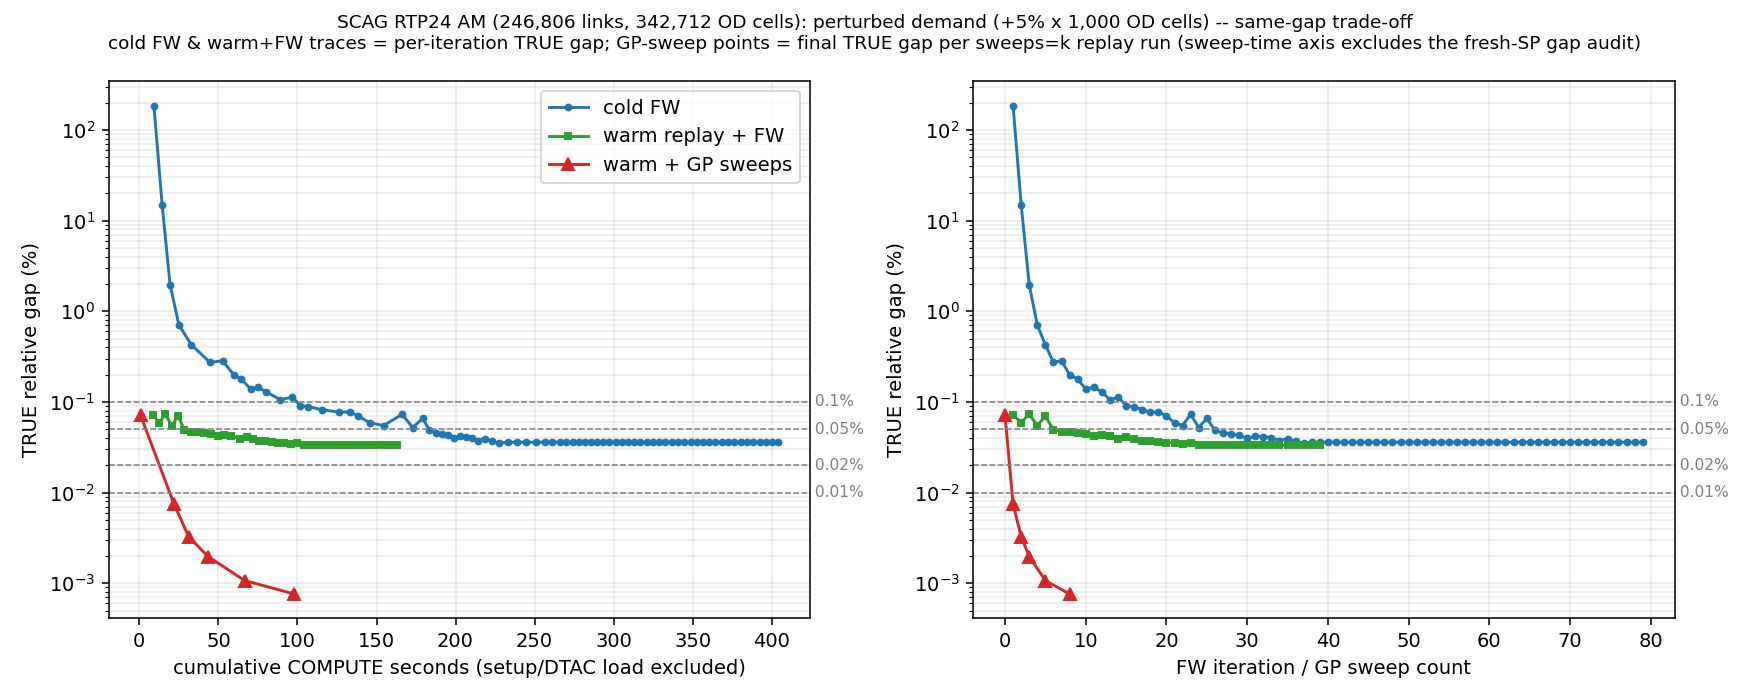
\includegraphics[width=\textwidth]{l3_tradeoff_scag.png}
\caption{SCAG RTP24 AM same-gap trade-off. Left: TRUE relative gap vs
cumulative compute seconds (setup/DTAC load excluded); right: vs FW
iteration / GP sweep count. FW curves are per-iteration TRUE gap; GP points
are the final TRUE gap of each sweeps$=k$ run. Companion figure
\code{l3\_tradeoff\_sketch.png} shows the same regimes on Chicago Sketch
(0.10\% $\to$ 4.8x, 0.05\% $\to$ 2.4x, 0.02\%/0.01\% $\to$ GP only).}
\label{fig:samegap}
\end{figure}

\textbf{The regime split} is the finding of Figure~\ref{fig:samegap}: plain
FW --- cold \emph{or} warm-started --- plateaus above $\sim$0.03\% on these
networks, while GP sweeps over the stored columns pass 0.01\% in 1--3 sweeps
and keep going (SCAG, 8 sweeps: $7.6\times10^{-4}$\,\%). The sweeps are not
merely faster to a fixed target; they reach targets FW cannot. Their cost
scales with OD count (SCAG 343k ODs: $\sim$23\,s first sweep, $\sim$11\,s
after; Chicago Regional 2.3M ODs: $\sim$60\,s), which motivates the remaining
per-origin parallelization work.

\begin{center}
\fbox{\begin{minipage}{0.93\textwidth}
\textbf{The standard rerun recipe (team decision).} Rerunning \emph{any}
model = L3 column warm start with a 0.1\% relative-gap target:
\begin{center}
\code{warm\_start\_columns = route\_columns.bin} \quad
\code{convergence\_gap\_pct = 0.1} \quad
\code{column\_adjust\_sweeps = 0}
\end{center}
(the baseline run sets \code{column\_output=1} once). Replay+FW reaches the
0.1\% TRUE gap in $\sim$1 iteration --- on SCAG, 139x less compute than a cold
run to the same gap. Add GP sweeps only for tighter targets (1 sweep reaches
0.01\% on SCAG). Kernel cold-start defaults are unchanged; the recipe is
settings-only. Full recipe and guard behavior:
\code{github\_taplite/docs/RERUN\_RECIPE.md}.
\end{minipage}}
\end{center}

\section{The binary format family}

\begin{table}[h]
\centering
\caption{TAPLite binary formats. All carry magic + version headers, match by
external link id, and fall back loudly (never fail) on invalid input.}
\label{tab:formats}
\begin{tabular}{llll}
\toprule
Magic & Role & Written by & Consumed by \\
\midrule
DTAB & OD demand input & \code{dtalite\_qa demand-bin} & \code{demand\_format=1} (2.5--3x faster load) \\
DTLP & Link performance & \code{link\_output=3} & L1 \code{warm\_start\_times}; reporting \\
DTLR & Flow restart snapshot & \code{flow\_snapshot=1} & L2 \code{warm\_start\_flows} \\
DTAC & Path/column store (v2: $\theta$ shares) & \code{column\_output=1} & verifier; L3 \code{warm\_start\_columns} \\
DTST & Full state snapshot & \emph{planned} (L4) & \emph{planned}: mmap, skips input parse \\
\bottomrule
\end{tabular}
\end{table}

\section{Engineering principles}
\label{sec:principles}

The efficiency track is governed by rules that came directly out of the panel
and are enforced on every increment:

\begin{itemize}[nosep]
  \item \textbf{Exact or clearly reported.} A feature is either bit-exact
    (P0 trio, L2 under a matching fingerprint) or its deviation is quantified
    and printed (DTAC increment-1 $R^2$; the future restricted-vs-full gap split).
  \item \textbf{Default-off.} Every behavior-changing key
    (\code{warm\_start\_times}, \code{warm\_start\_flows}, \code{flow\_snapshot},
    \code{column\_output}) defaults off and is registered in the
    \code{dtalite\_qa} schema; existing runs are byte-identical.
  \item \textbf{Loud-warn, never fail.} Bad warm-start input --- missing file,
    wrong magic, zero id matches, unmatched links from network edits --- warns
    loudly and degrades gracefully (cold start or L1 demotion); a production
    run is never aborted by an optimization hint.
  \item \textbf{Fingerprint guards.} Flow restarts are gated by an exact
    demand fingerprint; a single perturbed OD cell flips it. Grouping and
    warm-start decisions are always logged with match rates.
  \item \textbf{Regression + byte-identity gates.} Every increment must pass
    the 13-network / 30-check suite with \emph{no re-baselining}, plus
    byte-diffs of \code{link\_performance.csv} and gap trajectories against the
    pre-change executable.
  \item \textbf{No bush-based rewrite.} The panel unanimously rejected an
    Algorithm-B/TAPAS rewrite. The academic persona's framing: gradient-
    projection polish on stored columns delivers ``bush-method-class precision
    without becoming Algorithm~B'' --- disproportionate machinery for a
    single-file link-based FW kernel is exactly what this track avoids.
\end{itemize}

\section*{Summary}

P0, P1, and the full P2/L3 are shipped and verified: warm starts turn SCAG
reruns from a 185\%-gap cold open into a continuation that starts at the prior
final gap, and the L3 column store turns \emph{any} rerun --- including changed
demand --- into a 0.1\%-gap solution in $\sim$1 FW iteration (139x less compute
than cold on SCAG), with GP sweeps unlocking gap targets FW cannot reach at
all. The standard rerun recipe is now fixed: \code{warm\_start\_columns} +
\code{convergence\_gap\_pct=0.1} + zero sweeps, with zero change to any run
that does not opt in (30/30 regression, defaults-off byte-identity). Remaining
work: per-origin parallel GP sweeps (the serial sweeps dominate at
$\geq$2M ODs) and the L4 DTST state snapshot to kill the setup phase. The
ladder compounds: each rung reuses the formats and guards of the one below it.

\end{document}
